%%% Demographic Research Pandoc Style
%%%
%%% Jonas Schöley
%%% jschoeley@gmail.com
%%%
%%% 2021-02-19
%%%
%%% Depends on file "drbibstyle.bst" for custom bibliography styling,
%%% "drtitling" for title formating,
%%% "drlogo.pdf" for the Demographic Research logo.
%%%
%%% Based upon the work of
%%% Jana Korsinek
%%% Peter Wilhelm
%%% Peter Wilson
%%% and very probably others such as the countless student assistants
%%% who, over the years, worked at Demographic Research.

%--- Documentclass -----------------------------------------------------

\documentclass[10pt,twoside,reqno]{article}
\raggedbottom

%--- Font/encoding -----------------------------------------------------

\usepackage[utf8]{inputenc} % .tex-file text encoding
\usepackage[T1]{fontenc}    % vector fonts and special chars in output
\usepackage{times}          % Times Roman font family

%--- Constants ---------------------------------------------------------

% provided by YAML header of markdown file

% document title
  \def \thetitle {The impact of population heterogeneity
on the age trajectory of neonatal mortality:
a study of US births 2008-2014}
  \def \theshorttitle {The impact of population heterogeneity on the age trajectory of neonatal mortality}

% first page of document in volume
  \def \thestartpage {1}

% article and volume numbers
  \def \thearticle {xx}
  \def \thevolume {XX}

% date of publication
  \def \thedatepub {day month 2025}

% category of article
  \def \thecat {Research article}

% publication blurb

% author listings
  \def \theheadingauthor {Schöley}

% number of authors
\newcounter{authorcount}
   \stepcounter{authorcount} 

%--- Maths -------------------------------------------------------------

\usepackage{amsmath}  % various maths features
\usepackage{amssymb}  % maths symbols
\usepackage{mathrsfs} % maths script fonts

%--- Misc --------------------------------------------------------------

\usepackage{etoolbox} % allows to inject commands inside environments
\usepackage{placeins} % control the placement of floats via \FloatBarrier
\usepackage{xcolor}   % for colored links

%--- Figures -----------------------------------------------------------


  \usepackage{graphicx} % include external images

  % generate all images so they have a width \cnstmaxfigwidth
  % images get their normal width if they fit onto the page
  % images are scaled down if they would overflow the margins
  \makeatletter
    \def\cnstmaxfigwidth{
      \ifdim \Gin@nat@width>\linewidth
        \linewidth
      \else \Gin@nat@width
      \fi
    }
  \makeatother
  \let\Oldincludegraphics\includegraphics
  \renewcommand{\includegraphics}[1]{\Oldincludegraphics[width=\cnstmaxfigwidth]{#1}}

  \AfterEndEnvironment{figure}{\FloatBarrier}


%--- Captions ----------------------------------------------------------

% define caption style
\usepackage[hang]{caption}
\DeclareCaptionLabelSeparator{capsep}{:}
\DeclareCaptionFormat{capformat}{#1#2\hspace{1cm}#3}
\DeclareCaptionFont{capfont}{\normalsize\bfseries}
\captionsetup[figure]{
            style           = default,
            indention       = 2.4cm,
            labelsep        = capsep,
            format          = capformat,
            name            = Figure,
            font            = capfont,
            labelfont       = capfont,
            justification   = raggedright,
            singlelinecheck = false
}
\captionsetup[table]{
            style           = default,
            indention       = 2.25cm,
            labelsep        = capsep,
            format          = capformat,
            name            = Table,
            font            = capfont,
            labelfont       = capfont,
            justification   = raggedright,
            singlelinecheck = false
}

% captions above
\usepackage{float}
\floatstyle{plaintop}
\restylefloat{table}
\restylefloat{figure}

%--- Localization ------------------------------------------------------

% babel
\usepackage[english]{babel} % document language/localization
\usepackage{hyphenat}       % hyphenation rules

% hyphenation rules for specific words
  \hyphenation{de-mo-gra-phic Bayesian}

%--- Links -------------------------------------------------------------

\usepackage{hyperref}
\hypersetup{
  hidelinks=true,
  breaklinks=true,
  colorlinks=false,
  pdftitle={\thetitle}
}
\urlstyle{rm}

%--- Bibliography ------------------------------------------------------

\usepackage{natbib}
\bibpunct [: ] {(} {)} {;} {a} {} {,}
\setcitestyle{aysep={}}
\bibliographystyle{drbibstyle}
% special doi and url format in bibliography (used in .bst file)
\newcommand{\doi}[1]{\href{https://www.dx.doi.org/#1}{\textcolor{blue}{doi:#1}}}
    % use url command to escape special chars in url
\newcommand{\biburl}[1]{\href{#1}{\textcolor{blue}{\url{#1}}}}
    % which url prefix to use
\newcommand{\urlprefix}{}

%--- General layout ----------------------------------------------------

% page layout
\usepackage{geometry}
\geometry{
  paperheight = 22cm,
  paperwidth  = 17cm,
  top         = 2.54cm,
  bottom      = 2.54cm,
  inner       = 2cm,
  outer       = 2.54cm,
  footskip    = 11mm,
  headheight  = 1cm,
  headsep     = 0.75cm,
  showframe   = false
}

% title and cover format
\usepackage{drtitling}

% spacing
\setlength{\parskip}{0ex}
\setlength{\parindent}{.7cm}
\setlength{\bibsep}{.18cm}
\setlength{\belowdisplayskip}{15pt} \setlength{\belowdisplayshortskip}{10pt}
\setlength{\abovedisplayskip}{15pt} \setlength{\abovedisplayshortskip}{10pt}

% avoid orphans and widows
\widowpenalty = 10000
\clubpenalty  = 10000

% don't break footnotes
\interfootnotelinepenalty = 10000

% don't hyphenate across pages
\brokenpenalty10000\relax

%--- Lists -------------------------------------------------------------

% tight lists
\providecommand{\tightlist}{%
  \setlength{\topsep}{0pt}
  \setlength{\partopsep}{0pt}
  \setlength{\itemsep}{0pt}
  \setlength{\parsep}{.9\parskip}
}
\makeatletter
  \def\@listI{%
    \leftmargin\leftmargini } \let\@listi\@listI \@listi
  \def\@listii{%
    \leftmargin\leftmarginii
    \labelwidth\leftmarginii  \advance \labelwidth-\labelsep
    }
\def\@listiii{%
    \leftmargin\leftmarginiii
    \labelwidth\leftmarginiii  \advance \labelwidth-\labelsep
    }
\makeatother

%--- Sections ----------------------------------------------------------

% section spacing
\makeatletter
\renewcommand\section{\@startsection {section}{1}{\z@}%
                                   {-24pt}%
                                   {2.3ex \@plus.2ex}%
                                   {\normalfont\large\bfseries}}
\renewcommand\subsection{\@startsection{subsection}{2}{\z@}%
                                     {-24pt}%
                                     {1.5ex \@plus .2ex}%
                                     {\normalfont\normalsize\bfseries}}
\makeatother

% section style
\usepackage[nobottomtitles]{titlesec}
\titleformat{\section}[hang]{\raggedright\normalfont\bfseries\large}{\arabic{section}.}{1ex}{}
\titleformat{\subsection}[hang]{\raggedright\normalfont\bfseries}{\arabic{section}.\arabic{subsection}}{1ex}{}
\titleformat{\subsubsection}[hang]{\raggedright\normalfont\bfseries}{\arabic{section}.\arabic{subsection}.\arabic{subsubsection}}{1ex}{}

%--- Table of content --------------------------------------------------

% table of content format
\makeatletter
\renewcommand*{\@pnumwidth}{3em} % width of toc page number box
\renewcommand*\l@section[2]{%
  \ifnum \c@tocdepth >\z@
    \addpenalty\@secpenalty
    \addvspace{1.0em \@plus\p@}%
    %\setlength\@tempdima{1.5em}%
    \setlength\@tempdima{4em}%
    \begingroup
      \parindent \z@ \rightskip \@pnumwidth
      \parfillskip -\@pnumwidth
      \leavevmode %\bfseries
      \advance\leftskip\@tempdima
      \hskip -\leftskip
      #1\nobreak\hfill \nobreak\hb@xt@\@pnumwidth{\hss #2}\par
    \endgroup
  \fi}
\renewcommand*\l@subsection[2]{%
  \ifnum \c@tocdepth >\z@
    \addpenalty\@secpenalty
    %\addvspace{1.0em \@plus\p@}%
    %\setlength\@tempdima{1.5em}%
    \setlength\@tempdima{4em}%
    \begingroup
      \parindent \z@ \rightskip \@pnumwidth
      \parfillskip -\@pnumwidth
      \leavevmode %\bfseries
      \advance\leftskip\@tempdima
      \hskip -\leftskip
      #1\nobreak\hfill \nobreak\hb@xt@\@pnumwidth{\hss #2}\par
    \endgroup
  \fi}
\renewcommand*\l@subsubsection[2]{%
  \ifnum \c@tocdepth >\z@
    \addpenalty\@secpenalty
    %\addvspace{1.0em \@plus\p@}%
    %\setlength\@tempdima{1.5em}%
    \setlength\@tempdima{4em}%
    \begingroup
      \parindent \z@ \rightskip \@pnumwidth
      \parfillskip -\@pnumwidth
      \leavevmode %\bfseries
      \advance\leftskip\@tempdima
      \hskip -\leftskip
      #1\nobreak\hfill \nobreak\hb@xt@\@pnumwidth{\hss #2}\par
    \endgroup
  \fi}
\makeatother

%--- Header ------------------------------------------------------------

% define the specific headers and footers to be added to each page

\usepackage{fancyhdr} % page headers
\pagestyle{empty}

% use short title of title is too long for header
\newlength{\testlaenge}
\settowidth{\testlaenge}{\footnotesize\emph{\theheadingauthor}: \thetitle}
\ifdim410pt<\testlaenge
  \edef\theheadingtitle{\theshorttitle}
\else
  \edef\theheadingtitle{\thetitle}
\fi

\def\drfootersize{\footnotesize}   % size of footer font
\renewcommand{\headrulewidth}{0pt} % no headrule

% some latex commands such as ´\maketitle´ automatically run
% \pagestyle{plain}. this redefines pagestyle "plain" so that nothing
% is added to header or footer
\fancypagestyle{plain}{
  \fancyhf{}
}

% header and footer regular text
\fancypagestyle{regular}{
  \fancyhf{}
  \fancyhead[LE]{\footnotesize\emph{\theheadingauthor}: \theheadingtitle} \chead{}
  \fancyhead[RO]{\footnotesize \emph{Demographic Research}: Volume \thevolume, Article \thearticle}
  \fancyfoot[RO,LE]{\drfootersize \arabic{page}} \cfoot{}
  \fancyfoot[LO,RE]{\drfootersize\href{https://www.demographic-research.org}{https://www.demographic-research.org}}
}
% header and footer on title page
\fancypagestyle{title}{
  \fancyhf{}
  \fancyhead[LO]{}
  \fancyhead[RO]{}
  \fancyhead[CO,CE]{\footnotesize \emph{Demographic Research}: Volume \thevolume, Article \thearticle\\[1mm]\emph{\thecat}}
  \fancyfoot[RO,LE]{\drfootersize \arabic{page}} \cfoot{}
  \fancyfoot[LO,RE]{\drfootersize\href{https://www.demographic-research.org}{https://www.demographic-research.org}}
}

%--- Footnotes ---------------------------------------------------------

\usepackage[bottom]{footmisc}

% make linebreaks start under footnote label
\setlength{\footnotemargin}{0.3em}
% move footnoterule to the right
\makeatletter
  \let\oldfootnoterule=\footnoterule
  \def\footnoterule{\moveright0.8cm\vbox{\oldfootnoterule}}
\makeatother

\let\oldfootnote\footnote
\renewcommand\footnote[1]{%
\oldfootnote{\hspace{0.6mm}#1}}

% if you have code in your footnotes, the million macro march
% kind of bumps into itself.
% Pandoc, having just rendered your text into LaTeX,
% knows whether the 'variable' `verbatim-in-note` is True, and
% If it is, it asks for a  LaTeX package that solves the dilemma:
%
%--- Code listings -----------------------------------------------------


%--- Tables ------------------------------------------------------------

  \usepackage{array,longtable,booktabs,multirow}
  % -- This is needed because raggedright in table elements redefines \\:
  \newcommand{\PreserveBackslash}[1]{\let\temp=\\#1\let\\=\temp}
  \let\PBS=\PreserveBackslash

  % https://tex.stackexchange.com/a/503439
  \makeatletter
  \let\tableorig\table
  \def\table@i[#1]{\tableorig[#1]\scriptsize\sffamily}  % with optional argument
  \def\table@ii{\tableorig\scriptsize\sffamily}  % without optional argument
  \def\table{\@ifnextchar[\table@i \table@ii}  % Redefine depending on presence of [
  \makeatother


  \AfterEndEnvironment{table}{\FloatBarrier}


%--- Subscripts --------------------------------------------------------


%--- Includes ----------------------------------------------------------

% header_includes
  \usepackage{booktabs}
  \usepackage{longtable}
  \usepackage{array}
  \usepackage{multirow}
  \usepackage{wrapfig}
  \usepackage{float}
  \usepackage{colortbl}
  \usepackage{pdflscape}
  \usepackage{tabu}
  \usepackage{threeparttable}
  \usepackage{threeparttablex}
  \usepackage[normalem]{ulem}
  \usepackage{makecell}
  \usepackage{xcolor}

%--- Title -------------------------------------------------------------

\expandafter\title\expandafter{\expandafter\textbf\expandafter{\thetitle}\vspace{5mm}}

%--- Authors -----------------------------------------------------------

% for title
  \author{\textbf{Jonas Schöley}
    \thanks{\hspace*{.28ex}Max Planck Institute for Demographic Research, Rostock, Germany. \href{}{\color{blue}\href{mailto:schoeley@demogr.mpg.de}{\nolinkurl{schoeley@demogr.mpg.de}}}.}\vspace*{4mm}
  }

% for pdf metadata
  \def \themetaauthor { Jonas Schöley}
  \hypersetup{pdfauthor=\themetaauthor}

% for cover list
  \newcommand{\drcvrlistauthors}{
    \large{\textbf{Jonas\ Schöley}}
  }

% for copyright
  \newcommand{\drcvrcrauthors}{
    \copyright\ \normalsize{\emph{\the\year\ Jonas Schöley.}}
  }

%--- Print cover -------------------------------------------------------

\usepackage{lastpage}
\setcounter{page}{-1}
\newcommand{\drpages}{\thestartpage--\pageref*{LastPage}}

\newcommand{\makecover}{\begin{titlepage}%
  \begin{center}
    \Oldincludegraphics[width=11.5cm]{drlogo.pdf}
  \smallskip
  \rule{12cm}{1mm}\\
  \bigskip
  \bigskip
  \bigskip
  \begin{tabular}{p{8.5cm}}
    \fontfamily{ptm}\selectfont
    \large{\textbf{\emph{DEMOGRAPHIC RESEARCH}}}\\
    \bigskip
    \fontfamily{ptm}\selectfont\large{\textbf{VOLUME \thevolume, ARTICLE \thearticle, PAGES \drpages}}\\
    \fontfamily{ptm}\selectfont\large{\textbf{PUBLISHED \MakeUppercase{\thedatepub}}}\\
    \fontfamily{ptm}\selectfont\normalsize{\href{}{https://www.demographic-research.org/Volumes/Vol\thevolume/\thearticle/}}\\
    \fontfamily{ptm}\selectfont\normalsize{DOI: 10.4054/DemRes.\the\year.\thevolume.\thearticle}\\
    \medskip
    \fontfamily{ptm}\selectfont\large{\emph{\thecat}}\\
    \bigskip
    \begin{flushleft}
      \fontfamily{ptm}\selectfont\large{\textbf{{\raggedright\thetitle}}}
    \end{flushleft}
    \\[-0.4cm]
    %\bigskip
    \drcvrlistauthors
  \end{tabular}
  \vfill
  \begin{tabular}{p{8.5cm}}
      \drcvrcrauthors\\
    %\underline{\hspace*{4in}}
    \smallskip
    \begin{flushleft}\fontfamily{ptm}\selectfont\footnotesize{\emph{This open-access work is published under the terms of the Creative Commons Attribution 3.0 Germany (CC BY 3.0 DE), which permits use, reproduction, and distribution in any medium, provided the original author(s) and source are given credit.\\ See
    \href{https://creativecommons.org/licenses/by/3.0/de/legalcode}{https://creativecommons.org/licenses/by/3.0/de/legalcode}.}}
    \end{flushleft}
  \end{tabular}
  \end{center}
\end{titlepage}%
}

\begin{document}

\makecover

%--- Print TOC ---------------------------------------------------------

\newpage
\renewcommand{\contentsname}{Contents}
{\footnotesize \tableofcontents}

%--- Print title -------------------------------------------------------

\newpage
\setcounter{page}{\thestartpage}
\maketitle
\thispagestyle{title}

%--- Print abstract ----------------------------------------------------

\vspace*{-24pt}
\vspace*{5mm}
\setlength{\parskip}{0.5em}
\section*{Abstract}
  \noindent\textbf{BACKGROUND}\\
  The risk of death declines rapidly over the first month of life. It has been theorized that the fast pace of the decline is explained by hidden population heterogeneity resulting in a mortality selection process whereby the frailest infants leave the population at the fastest rate. A competing explanation situates the rapid mortality decline on the individual level, pointing towards the risky transition of birth and the subsequent adaptation of the newborn to the unfamiliar surroundings.
  \par
  \noindent\textbf{OBJECTIVE}\\
  To estimate heterogeneity in the level and shape of age-specific mortality within a cohort of newborns and to quantify the degree to which mortality selection explains the shape of the average neonatal mortality trajectory.
  \par
  \noindent\textbf{METHODS}\\
  Given individual-level data on 20,322,147 births and 82,562 neonatal deaths from the 2008-2012 U.S. birth cohort, I calculate life-tables for 252 mutually exclusive strata each defined by a unique combination of observed birth characteristics. Using this information, I characterize the distribution of mortality risk and its evolution over the first 28 days of life and decompose changes in key characteristics of this distribution -- the mean, the variance, and the mean-mode ratio -- into a mortality selection and a direct component.
  \par
  \noindent\textbf{RESULTS}\\
  The average age trajectory of neonatal mortality is highly influenced by a small group of frail newborns and does not reflect the rather flat age effect estimated for the healthy majority of the birth cohort. While the risk decline over the first day of life is substantially influenced by mortality selection, the overall age trajectory is better explained by the convergence of high-risk towards low-risk population strata.
  \par
  \noindent\textbf{CONTRIBUTION}\\
  I contribute an empirical test of the hypothesis that the age trajectory of mortality in the days and weeks following birth is an artifact of mortality selection.
\vspace*{12pt}

\setlength{\parskip}{0ex}

%--- Print main text ---------------------------------------------------

% start footnote numbering at <number of authors> + 1
\setcounter{footnote}{\value{authorcount}}
\newpage
\pagestyle{regular}

\section{Introduction}\label{introduction}

Never again throughout the existence of a cohort will the hazard of death change as rapidly as it does during the first few weeks following birth. For the 2009--2012 U.S. birth cohort, the risk of death falls tenfold over the first day of life, and again by a factor of ten over the next four weeks. But how reflective is this population-level phenomenon of a single newborn's risk trajectory? Is the period of exceptional risk right after birth part of every human's experience, or have we been led astray by one more of ``Heterogeneity's Ruses'' \citep{Vaupel1985}? In this paper, I seek to quantify the impact of population heterogeneity on the age trajectory of neonatal mortality based on \emph{observed} mortality differences in a cohort of U.S. born infants.

Populations in which members are heterogeneous concerning their risk of death are subjected to mortality selection, which may be defined as the changing composition of a cohort over age due to heterogeneous mortality. As mortality is nothing but the rate of leaving a population due to death, with time, the proportion of low-mortality strata will increase, whereas strata with high mortality will become less prevalent. In consequence, any observed change of a cohorts trait over age (such as income, health, risk of death) may either be the result of within-stratum trait changes or result from a change in the cohort's composition along those strata over age due to mortality selection.

A rich (bio)demographic literature exists for the special case of mortality selection driving the shape of the population level hazard of death over age thus explaining phenomena such as late-life mortality plateaus \citep[e.g.,][]{Beard1959, Vaupel1979, Vaupel1993, Steinsaltz2006, Missov2015, Colchero2019}, the adolescent ``accident hump'' \citep{Remund2015}, declining mortality following surgery \citep{Hougaard1986} or the age pattern of early life mortality \citep{Vaupel1983, Hsieh1985, Trussell1985, Avraam2014}. All of the aforementioned literature features frailty models as a means to formalize, understand, and estimate the impact of population heterogeneity on the age trajectory of mortality. In these models, an individual's risk of death depends on a random quantity coined \emph{frailty} \citep{Vaupel1979} that, on account of being unobserved, may be thought of as hidden heterogeneity between members of a cohort. Frailty is most commonly expressed in a proportional hazards framework where the hazard of death at age \(x\) of an individual with frailty \(z\) is given by \(h(x|z)=zh_0(x)\) and \(h_0(x)\) is a \emph{baseline hazard} shared by all members of the population. An expression for the population/marginal/unconditional hazard \(\overline{h}(x)\) can be derived\footnote{An excellent introduction to this technique can be found in \citet{Wienke2011}.} by assuming a distribution of survival times for the case where \(z=1\) with corresponding hazard \(h_0\) and a distribution for the frailties at age \(x=0\). It is then possible to fit \(\overline{h}(x)\) to observed survival times or a life table and -- given the parameters of the fit and an array of formal relationships \citep{Vaupel1983, Vaupel2014} -- to determine how hidden heterogeneity acts in the population under investigation. Herein lies one central attraction of frailty models: they allow inference about population heterogeneity even if none has been observed. The quality of the inference then, of course, crucially depends on the adequacy of the assumptions going into the model.

\begin{figure}
\centering
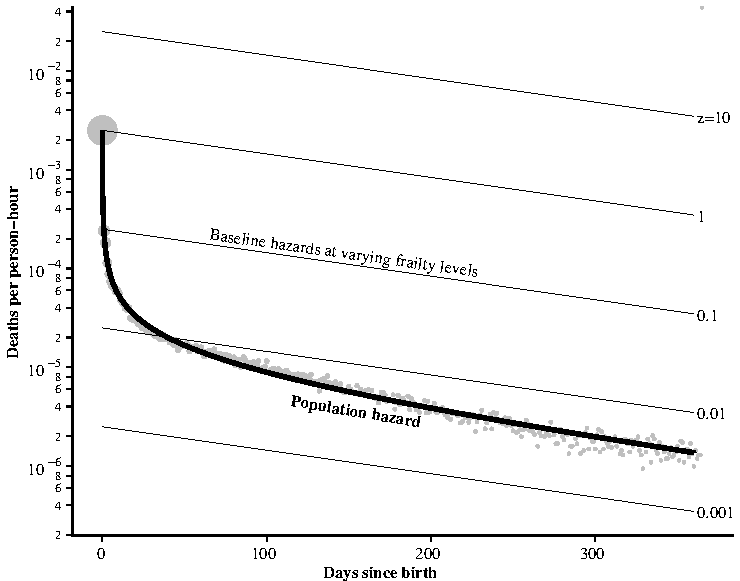
\includegraphics{fig/hougaard_gompertz_fit.pdf}
\caption{\label{fig:hougaard-gompertz-fit}Predicted hazard (black) vs.~life table mortality rates (gray) for the 2008--2012 U.S. birth cohort. Daily mortality rates over the first 365 days of life are well described by a Gompertz baseline distribution with Hougaard distributed frailties. Via the process of mortality selection, a mixture of log-linear individual level hazards, here drawn for various levels of frailty \(z\), gives rise to a population level hazard with extreme curvature on the log scale. The area of the circles is in rough proportion to the number of deaths each day.}
\end{figure}

A frailty explanation for the age trajectory of mortality following birth has been put forward multiple times in the literature but never seriously followed up upon. \citet{Vaupel1983} modeled the hazard of infant death, assuming a constant baseline hazard and multiplicative Gamma distributed frailty with unity mean and a variance of 500. Such a model implies that the majority of infants at birth are at virtually no risk of death with a small minority of critical cases\footnote{A Gamma distribution with unity mean and variance 500 has more than 98.8 percent of its probability mass below the mean and 0.24 percent at least 100 times above.}. \citet{Trussell1985} demonstrated how sensitive the choice of baseline hazard is when modeling infant mortality via a frailty model, with the Gompertz leading to decreasing and the Weibull to increasing individual-level risk trajectories. \citet{Hougaard1984} hypothesized that the high mortality during the first year of life and the subsequent rapid decline might be the result of an ``extreme frailty distribution'' upon birth, meaning a distribution with a long right tail, and he proposed the inverse-Gamma distribution as a suitable candidate. \citet{Hougaard1986} introduced a particularly flexible family of frailty distributions, including the Gamma, the inverse-Gaussian, and distributions derived from the positive-stable. He fitted a corresponding frailty model to data on time until death after myocardial infarct, a survival scenario not unlike the neonatal case as there is a stressor at time zero with mortality declining quickly and monotonically thereafter.

Indeed the Hougaard frailty model with a Gompertz baseline hazard (see Appendix A for the model specification) gives an excellent fit not only to neonatal mortality but to the entire day-to-day infant life table of the 2009--2012 U.S. birth cohort, capturing the extremely steep decrease in hazard following birth and the subsequent log-linear decline during the post-neonatal period (Figure \ref{fig:hougaard-gompertz-fit}). While by no means a proof of the frailty hypothesis, this simple model shows that a mortality selection explanation is consistent with the dynamics of daily mortality rates observed on the population level.

More recently, the heterogeneous frailty hypothesis was discussed by \citet{Levitis2011} and \citet{Levitis2013} as an alternative to evolutionary explanations for ``ontogenescence,'' i.e., the declining hazard of death following birth observed in many species. Via simulation Levitis demonstrated how age-independent individual-level risk leads to age-dependent population mortality rates. In a further variation on the theme, \citet{Avraam2014} captured the decline in mortality from birth to adolescence by employing a discrete frailty model with subgroups featuring either exponentially increasing or constant hazards.

Without data on heterogeneous risks, the hypothesis of mortality selection can only be tested indirectly. While frailty models do provide heterogeneity estimates from population-level data alone, this can only be taken as suggestive evidence for a selection explanation. The estimated amount of heterogeneity depends crucially on the choice of baseline hazard, the choice of frailty distribution, the assumption of fixed versus changing frailty, and the specific way that frailty modulates the baseline hazards (proportional hazards vs.~accelerated failure time). These assumptions can not be validated on population-level data as different model specifications yield the same parametric form for the marginal hazard \citep{Trussell1985, Hoem1990, Yashin2000}. I argue that a more convincing case for the impact of population heterogeneity on the age trajectory of mortality can be made by analyzing the distribution of risk in a cohort stratified by \emph{observed} characteristics. For infants, such data is available on birth certificates.

A birth certificate contains a wealth of information that identifies potentially frail newborns. Routinely collected are birth weight, the length of pregnancy, and the Apgar score, an index of the vitality of the child shortly after delivery. The combination of these characteristics delineates hundreds of highly specific subpopulations within a single birth cohort and, based on the distribution of deaths and exposure times across these strata, I analyze the impact of population heterogeneity on the age trajectory of neonatal mortality using both discrete-time life table decomposition methodology and continuous-time hazard modeling in connection with results from formal demography. This approach of describing mortality selection along observed mortality differentials has little precedence as far as human mortality is concerned, an exception being \citet{Remund2015} who, based on an analysis of French individual level survival data with covariates, found that selection effects contribute to the ``accident hump'' observed in the hazard trajectory of young adults.

Following the description of the U.S. 2008--2012 birth cohort, I outline a discrete life table approach and a complementary continuous time hazard method to quantify population heterogeneity and mortality selection and its impact on the age trajectory of neonatal mortality. This is followed by results on the distribution of neonatal mortality risks as it changes over age, the heterogeneity of hazard trajectories, and various decompositions of population-level statistics along the age dimension. A discussion of the results concludes the paper.

\section{Data}\label{data}

As population heterogeneity drives mortality selection, one can learn about selection effects by estimating the hazard of death across a diverse collection of population strata. Such estimation is possible given the publicly available ``NCHS Cohort Linked Birth -- Infant Death Data Files'' \citep{NCHS2016} which contain a complete census of births and infant deaths on the territory of the United States (excluding overseas territories) and feature most fields present on the birth and death certificates. The size and detail of the data allow the calculation of neonatal life tables over hundreds of subpopulations, capturing observed heterogeneity in mortality following birth.

To increase the sample size and thus the reliability of the stratum specific mortality estimates, I pool births and deaths across cohorts 2008 to 2012. This leaves a sample size of 20,322,147 births contributing 567,031,738 person-days of exposure to risk over the first 28 days of life, during which 82,562 neonatal deaths were registered.

Following the practice of statistical offices, I compute mortality rates based on \emph{all} registered births and deaths, including cases with missing data on key birth characteristics and unreasonable covariate combinations (e.g., extremely preterm delivery with average birth weight). While this approach challenges any causal interpretation of the determinants of neonatal death, it allows one to capture, in great detail, the observed heterogeneity giving rise to the usual population-level estimates. For this paper, it is of no concern whether the relationship between observed characteristics at birth and risk of death is causal or not as the phenomenon of interest -- mortality selection -- is induced by any mortality differential between population strata, no matter the cause.

For stratification, I use the information on birth weight, age of gestation at delivery, and 5 minute Apgar score. These variables are routinely recorded upon birth and highly predictive of neonatal death \citep{Pollack2000, Casey2001, Park2018}. As the inclusion of further strata only contributes minimal additional heterogeneity compared to what is already captured by the Apgar-birth weight-prematurity trias but considerably increases the computational demands of the model fitting procedure, I opted against it.

The variables are defined and discretized as follows:

\begin{description}
\tightlist
\item[Gestation at delivery alias prematurity]
The number of weeks from conception to delivery commonly estimated by the time since the first day of the mother's last menstrual cycle plus 14 days. Discretized into five groups \emph{Extremely preterm} (earlier than 28 weeks), \emph{Very preterm} (28 to 32 weeks), \emph{Moderate to late preterm} (32 to 37 weeks), \emph{Term or post-term} (37 weeks or later), and \emph{Missing}.
\item[Birth weight]
The weight of the newborn child measured in the minutes following birth discretized into the five categories \emph{Extremely low} (\textless1000g), \emph{Very low} (1000--1500g), \emph{Low} (1500--2500g), \emph{Regular or high} (2500g and above) and \emph{Missing}.
\item[5 minute Apgar score]
A measure of the infant's physical condition five minutes following birth, based on muscle activity, pulse, response to stimulation, skin color, and respiration of the newborn \citep{Apgar1953}. Vitality increases over integers zero to ten, with missings being treated explicitly as a twelfth category.
\end{description}

Table \ref{tab:tab-summary} shows births, death counts, and empirical 28-day survival for the complete 2008 to 2012 birth cohort by level of gestation, birth weight, and Apgar score, respectively.

\begin{table}[!h]
\centering
\caption{\label{tab:tab-summary}Summary statistics of the U.S. 2008--2012 birth cohort.}
\centering
\begin{tabular}[t]{rrrrrr}
\toprule
 & Births & (\%) & Deaths & (\%) & \% 28 day survival\\
\midrule
\addlinespace[0.3em]
\multicolumn{6}{l}{\textbf{Total}}\\
\hspace{1em} & 20,322,147 & (100.0) & 82,562 & (100.0) & 99.5\\
\addlinespace[0.3em]
\multicolumn{6}{l}{\textbf{5 minute Apgar score}}\\
\hspace{1em}\hspace{1em}0 & 9,981 & (0.1) & 5,154 & (6.3) & 48.3\\
\hspace{1em}1 & 45,091 & (0.3) & 28,430 & (34.5) & 36.9\\
\hspace{1em}2 & 30,569 & (0.2) & 9,839 & (12.0) & 67.8\\
\hspace{1em}3 & 31,941 & (0.2) & 4,987 & (6.1) & 84.3\\
\hspace{1em}4 & 43,408 & (0.3) & 3,705 & (4.5) & 91.4\\
\hspace{1em}5 & 72,970 & (0.4) & 3,781 & (4.6) & 94.8\\
\hspace{1em}6 & 135,842 & (0.7) & 4,456 & (5.4) & 96.7\\
\hspace{1em}7 & 364,256 & (1.8) & 5,119 & (6.3) & 98.5\\
\hspace{1em}8 & 2,017,526 & (10.0) & 5,577 & (6.8) & 99.7\\
\hspace{1em}9 & 16,746,692 & (82.5) & 7,869 & (9.6) & 99.9\\
\hspace{1em}10 & 715,842 & (3.6) & 242 & (0.3) & 99.9\\
\hspace{1em}(Missing) & 108,029 & (0.6) & 3,403 & (4.2) & 96.8\\
\addlinespace[0.3em]
\multicolumn{6}{l}{\textbf{Gestation at delivery}}\\
\hspace{1em}Extremely preterm & 149,760 & (0.8) & 50,606 & (61.3) & 66.2\\
\hspace{1em}Very preterm & 246,770 & (1.3) & 6,990 & (8.5) & 97.1\\
\hspace{1em}Moderate to late preterm & 2,029,693 & (10.0) & 9,484 & (11.5) & 99.5\\
\hspace{1em}Term or post-term & 17,870,545 & (88.0) & 14,493 & (17.6) & 99.9\\
\hspace{1em}(Missing) & 25,379 & (0.2) & 989 & (1.2) & 96.1\\
\addlinespace[0.3em]
\multicolumn{6}{l}{\textbf{Birth weight}}\\
\hspace{1em}Extremely low & 146,303 & (0.8) & 52,350 & (63.5) & 64.2\\
\hspace{1em}Very low & 151,709 & (0.8) & 5,692 & (6.9) & 96.2\\
\hspace{1em}Low & 1,355,547 & (6.7) & 10,573 & (12.9) & 99.2\\
\hspace{1em}Regular or high & 18,663,662 & (91.9) & 13,363 & (16.2) & 99.9\\
\hspace{1em}(Missing) & 4,926 & (0.1) & 584 & (0.8) & 88.1\\
\bottomrule
\end{tabular}
\end{table}

\section{Methods}\label{methods}

From neonatal life tables stratified by birth characteristics, I derive the empirical distribution of mortality rates conditioned on time since birth for a cohort of newborns. Age differences in three key characteristics of this distribution -- the mean, the variance, and the mean to mode ratio -- are then decomposed into components due to mortality selection and due to ``direct'' effects. Adopting a continuous-time perspective, I estimate hazard trajectories and survival curves for every subpopulation and a corresponding population hazard. By employing the Vaupel-Zhang equality, I calculate the degree to which the between-stratum variance in hazard rates compounds the slope of the population hazard at selected exact ages.

\subsection{Stratified infant life-tables}\label{stratified-infant-life-tables}

Consider a cohort of \(i=1,\ldots,N\) newborns stratified into subpopulations \(k=1,\ldots,K\) according to the combined discrete characteristics birth weight, age of gestation at birth and five minute Apgar score. Observed for every newborn are a survival time \(t_{ik}\) in days since birth censored at day 28 and a binary death indicator \(\delta_{ik}\). I partition the survival time into \(j=1,\ldots,J\) non-overlapping daily age intervals \([x_j, x_j+1)\), where \(x_j\) is the start of the \(j\)th age interval, and for each interval calculate stratum specific death counts \({D_{jk}=\sum_{i}\delta_{ijk}}\), population alive at the beginning of the age interval

\[
N_{jk}=\begin{cases}\text{Births}_k & \text{for}\,j=1\\ \text{Births}_k-\sum^{s=j}_{s=1}D_{j=s,k} & \text{for}\,j>1\end{cases},
\]

and person-days of exposure \(E_{jk}=N_{j+1,k}+a_{jk}D_{jk}\), with \(a_{jk}\) as the average time of death of those dying in age interval \(j\). For the first day of life I calculate \(a_j\) using information on the proportion of deaths during the first hour of life while for the other days the usual mid-point assumption \(a_{jk}=0.5\) is employed. I then calculate stratum specific life table death rates \(m_{jk}=\frac{D_{jk}}{E_{jk}}\) for each age interval and corresponding population level death rates \(\overline{m}_j=\frac{\sum_k D_{jk}}{\sum_k E_{jk}}\) and relative exposures \(p_{jk} = \frac{E_{jk}}{\sum_k E_{jk}}\). These tabulated counts, exposures, rates and proportions form the basis of all subsequent analyses.

\subsection{Discrete-time life table analysis}\label{discrete-time-life-table-analysis}

\subsubsection*{Decomposing change in mean mortality over age}\label{decomposing-change-in-mean-mortality-over-age}
\addcontentsline{toc}{subsubsection}{Decomposing change in mean mortality over age}

Using the shorthand \(\Delta f_x=f_{x+1}-f_x\) let \(\Delta \overline{m}_j\) denote the change in population-level mortality from age interval \(j\) to \(j+1\). How much of this difference is explained by a change of the subpopulation hazards and how much due to a change in the population composition induced by mortality selection? A straightforward solution to this decomposition problem can be derived by writing \(\overline{m}_j = \sum_kp_{jk}m_{jk}\) and applying the product rule for finite differences \citep{Boole1880} to the equivalent products \(m_{jk}p_{jk}=p_{jk}m_{jk}\) yielding the two expressions

\[
\begin{aligned}
  \Delta \overline{m}_j
  &= \sum_k p_{jk}\Delta m_{jk} + \sum_k m_{j+1,k} \Delta p_{jk} \\
  &= \sum_k m_{jk}\Delta p_{jk} + \sum_k p_{j+1,k} \Delta m_{jk},
\end{aligned}
\]

which when averaged give the well known Kitagawa decomposition \citep{Kitagawa1955},

\begin{equation}
  \Delta \overline{m}_j =
    \underbrace{
      \sum_k \frac{p_{jk}+p_{j+1,k}}{2}\Delta m_{jk}
    }_{
      \text{Direct change}~\Delta \overline{m}_j^D
    } +
    \underbrace{
      \sum_k \frac{m_{jk}+m_{j+1,k}}{2}\Delta p_{jk}
    }_{
      \text{Compositional change}~\Delta \overline{m}_j^C
    }.
\label{eq:decomp-rate}
\end{equation}

The two terms represent the change in the population mortality rate due to changes in the group-specific mortality rates and due to changing group composition. Of particular interest is the ratio \(\frac{\Delta \overline{m}_j^C}{\Delta \overline{m}_j}\), which for \(\Delta\overline{m}_j^C<0\) and \(\Delta \overline{m}_j<0\) is the share of the decline in population mortality explained by a compositional shift of the population. If mortality selection is indeed the main driver of the age decline in mortality over the neonatal period, then the aforementioned ratio has to be greater than 0.5.

\subsubsection*{Decomposing change in mortality rate variance over age}\label{decomposing-change-in-mortality-rate-variance-over-age}
\addcontentsline{toc}{subsubsection}{Decomposing change in mortality rate variance over age}

In addition to compounding the effect of age on the average risk of death, mortality selection can lower the variance of mortality rates across population strata as the survivors concentrate in more resilient subgroups. Alternatively, any change in population variance may result from stratum specific mortality rates converging over age. Because the variance of mortality rates across strata \(k\) among the survivors in age group \(j\) is the weighted average \(v_j(x)=\sum_k p_{jk}s_{jk}\), with \(s_{jk}=(m_{jk}-\overline{m}_{j})^2\), one can follow the same strategy as before to yield the Kitagawa-style decomposition

\begin{equation}
\Delta v_j =
  \underbrace{
    \sum_k \frac {p_{jk}+p_{j+1,k}} {2} \Delta s_{jk}
  }_{
    \text{Direct change}~\Delta v_j^D
  } +
  \underbrace{
    \sum_k \frac {s_{jk}+s_{j+1,k}} {2} \Delta p_{jk}
  }_{
    \text{Compositional change}~\Delta v_j^C
  },
\label{eq:decomp-var}
\end{equation}

with \(v_j^D\) denoting the change in variance due to convergence or divergence of stratum specific mortality rates over age towards the population mean and \(v_j^C\) the age-decline in variance due to changing population composition, i.e., mortality selection.

\subsubsection*{Decomposing change in the ratio of mean to modal mortality over age}\label{decomposing-change-in-the-ratio-of-mean-to-modal-mortality-over-age}
\addcontentsline{toc}{subsubsection}{Decomposing change in the ratio of mean to modal mortality over age}

If the distribution of death rates in a cohort of infants exhibits positive skewness, mortality selection can reduce the mean-mode ratio of this distribution by ``thinning the tail,'' i.e., by reducing the relative proportion of very frail subpopulations. However, any such decline may also result from genuine convergence of stratum specific death rates towards the death rates of the most prevalent stratum, the modal mortality rate, formally \(\mathscr{M}_j = m_{j,k=r}\) with \(r\) such that \(p_{j,k=r}=\text{max}(p_{j1},\ldots,p_{jK})\).

A Kitagawa-style decomposition of the mean-mode ratio \(\frac{\overline{m}_j}{\mathscr{M}_{j}} = \sum_k p_{jk}\frac{m_{jk}}{\mathscr{M}_j}\), shortened to \(r_j\), gives the two components

\begin{equation}
\Delta r_j =
  \underbrace{
    \sum_k \frac {p_{jk}+p_{j+1,k}} {2}
    \Delta \frac{m_{jk}}{\mathscr{M}_j}
  }_{
    \text{Direct change}~\Delta r_j^D
  } +
  \underbrace{
    \sum_k \frac {
      \frac{m_{jk}}{\mathscr{M}_j} + \frac{m_{j+1,k}}{\mathscr{M}_{j+1}}
    } {2}
    \Delta p_{jk}
  }_{
    \text{Compositional change}~\Delta r_j^C
  },
\label{eq:decomp-memora}
\end{equation}

where \(\Delta r_j^D\) captures the changing ratios of stratum specific mortality rates to modal mortality and \(\Delta r_j^C\) referring to changes in the population composition.

\subsection{Continuous-time hazard analysis}\label{continuous-time-hazard-analysis}

In the following, I outline a methodology to decompose the age derivative of the population hazard of death into a ``direct'' component reflecting actual age-effect within the population strata, and a ``compositional component'' capturing the confounding effect of population heterogeneity.

\subsubsection*{Estimating stratum specific hazard and survival}\label{estimating-stratum-specific-hazard-and-survival}
\addcontentsline{toc}{subsubsection}{Estimating stratum specific hazard and survival}

Stratum specific hazards during the neonatal period are well captured by the expression

\begin{equation}
  \begin{aligned}
    h_k(x) = e^{\beta_{0k} + \beta_{1k}\log(x+1) +
    \beta_{2k}\log^2(x+1)},
  \end{aligned}
\label{eq:lqhzrd}
\end{equation}

which can be interpreted as a Weibull hazard extended by a log-quadratic term over day of life (Appendix B). The curve has the advantage of being linear the log scale, thus allowing it to be fit as a generalized linear mixed/multilevel model, which greatly facilitates a stable estimation of stratum specific hazards. There are in total 252 strata in the population of newborns with each stratum \(k\) marking a unique combination of ``Prematurity,'' ``Birth weight,'' and ``Apgar score'' levels. Fitting the hazard separately to each stratum will result in erratic estimates as some strata do not contain enough observations to inform the model. A solution to this problem is to fit a multilevel model where instead of estimating \(\beta_{0k}, \beta_{1k}, \beta_{2k}\) directly one models the coefficient's distribution at different grouping levels.

Given the observed death counts \(D_{jk}\) in age group \(j\) and stratum \(k\) and associated person-days of exposure to risk \(E_{jk}\) I fit the model

\begin{equation}
  \begin{aligned}
    D_{jk} &\sim \text{Pois}\left(\lambda_{jk}E_{jk}\right) \\
    \lambda_{jk} &= e^{\beta_{0k} +
    \beta_{1k}\log(x_{jk}+1) +
    \beta_{2k}\log^2(x_{jk}+1)},
  \end{aligned}
\label{eq:themodel}
\end{equation}

where \(\lambda_{jk}\) are mortality rates by age group and stratum. For each stratum, a smooth hazard is recovered by evaluating \(\lambda_{jk}\) over a continuous range of ages \(x\) as in equation \eqref{eq:lqhzrd}.

The stratum specific coefficients \(\beta_{0k}\), \(\beta_{1k}\), \(\beta_{2k}\) are sums of baseline coefficients \(\beta\), prematurity effects \(\beta^\text{Pm}\), prematurity-birth weight interactions \(\beta^{\text{Pm}\times\text{Bw}}\), and prematurity-birth weight-Apgar interactions \(\beta^{\text{Pm}\times\text{Bw}\times\text{Ap}}\) resulting in the multilevel structure

\[
\left(\begin{aligned}
\beta_{0k} \\
\beta_{1k} \\
\beta_{2k}
\end{aligned}\right) =
\underbrace{\left(\begin{aligned}
\beta_0 \\
\beta_1 \\
\beta_2
\end{aligned}\right)}_{\substack{\text{lvl 0} \\ \text{ baseline coef.}}} +
\underbrace{\left(\begin{aligned}
\beta_{0,p[k]}^\text{Pm} \\
\beta_{1,p[k]}^\text{Pm} \\
\beta_{2,p[k]}^\text{Pm}
\end{aligned}\right)}_{\substack{\text{lvl 1} \\ \text{ deviations by} \\ \text{prematurity}}} +
\underbrace{\left(\begin{aligned}
\beta_{0,p[k],b[k]}^{\text{Pm}\times\text{Bw}} \\
\beta_{1,p[k],b[k]}^{\text{Pm}\times\text{Bw}} \\
\beta_{2,p[k],b[k]}^{\text{Pm}\times\text{Bw}}
\end{aligned}\right)}_{\substack{\text{lvl 2} \\ \text{ deviations by} \\ \text{birth weight given} \\ \text{prematurity}}} +
\underbrace{\left(\begin{aligned}
\beta_{0,p[k],b[k],a[k]}^{\text{Pm}\times\text{Bw}\times\text{Ap}} \\
\beta_{1,p[k],b[k],a[k]}^{\text{Pm}\times\text{Bw}\times\text{Ap}} \\
\beta_{2,p[k],b[k],a[k]}^{\text{Pm}\times\text{Bw}\times\text{Ap}}
\end{aligned}\right)}_{\substack{\text{lvl 3} \\ \text{ deviations by} \\ \text{Apgar given} \\ \text{prematurity and} \\ \text{birth weight}}},
\]

where \(p[k], b[k]\) and \(a[k]\) denote the prematurity, birth weight and Apgar level associated with stratum \(k\). Except for the baseline \(\beta\)'s each set of coefficients is assumed to be drawn from a multivariate-Normal distribution with zero mean and covariance matrix

\[
\Sigma = \begin{pmatrix}
    \sigma^2_{\beta_0} & \sigma_{\beta_0\beta_1} & \sigma_{\beta_0\beta_2} \\
    \sigma_{\beta_0\beta_1} & \sigma^2_{\beta_1} & \sigma_{\beta_1\beta_2} \\
    \sigma_{\beta_0\beta_2} & \sigma_{\beta_1\beta_2} & \sigma^2_{\beta_2}
    \end{pmatrix},
\]

with separate estimates for levels one to three.

Treating the coefficients as realizations from a multivariate-Normal distribution with zero mean acts as a regularizer on the estimated hazard trajectories. In cases where zero or very few deaths are observed, the stratum specific deviations will be ``pulled'' towards zero with the effect that the estimated hazard resembles the hazard of the next higher hierarchy level \citep{Gelman2007}. Take as an example the 303 infants delivered ``Very preterm'' with ``Very low'' birth weight and given an Apgar score of 10. Because all newborns survived the neonatal period, there is no information available to learn the shape of the underlying hazard. In the multilevel model, the larger population of infants delivered ``Very preterm'' with ``Very low'' birth weight will inform the hazard of the Apgar 10 subgroup. If plenty of data is available, then the hazard estimate will follow that data closely.

I fit model \eqref{eq:themodel} as a Generalized Linear Mixed Model using the \texttt{lme4} library in \texttt{R} \citep{Bates2015} and use the fitted coefficients to compute stratum specific hazard trajectories and survival curves -- the basis for the Vaupel-Zhang decomposition -- using the expressions given in Appendix C.

\subsubsection*{Vaupel-Zhang decomposition}\label{vaupel-zhang-decomposition}
\addcontentsline{toc}{subsubsection}{Vaupel-Zhang decomposition}

The Vaupel-Zhang equality \citep{Vaupel2010a} states that in any cohort stratified by some random characteristic \(K\) with initial distribution \(\pi_k = P(K=k)\) the age derivative of the average hazard of death amongst the survivors at age \(x\) can be written as

\[
  \dot{\overline{h}}(x) = \overline{\dot{h}}(x) - \sigma^2_h(x),
\]

where \(\overline{\dot{h}}(x)\) denotes average slope and \(\sigma^2_h(x)\) the average variance of hazards for the survivors at \(x\). This result can be interpreted as a decomposition of the slope in the population hazard at \(x\) into a direct and a compositional component: The first component is based upon the actual slopes of hazards within each stratum \(k\). Only if the population is completely homogeneous with respect to the levels of their hazards is the slope in the population hazard equal to the average slope in the stratum specific hazards. When, however, the variance of hazards is not zero, i.e., the population differs in their risk of death, mortality selection biases the slope in the population level hazard downwards. In other words, the trajectory of the population hazard over age is explained by the average hazard trajectory across population strata compounded by heterogeneity in the level of hazard.

The quantity of interest is the ratio \(\nu(x)=\frac{-\sigma_h^2(x)}{\dot{\overline{h}}(x)}\) which, given that \(\dot{\overline{h}}(x)<0\), is the share of decline in the population hazard at \(x\) explained by population heterogeneity in the level of mortality. From the observed distribution of birth characteristics \(\pi_k=\frac{\text{Births}_k}{\Sigma_k\text{Births}_k}\) and the estimated stratum specific hazards \(h_k(x)\) and survival \(S_k(x)\) I calculate the population survival curve \(S(x) = \sum_k \pi_k S_k(x)\) and the stratum distribution conditioned on survival to a given age \(\pi_k(x) = \frac{S_k(x)\pi_k}{S(x)}\) which in turn gives rise to the population hazard curve \(\overline{h}(x)= \sum_k \pi_k(x)h_k(x)\), and the variance of hazards over population strata \(\sigma^2_h(x) = \sum_k \pi_k(x) (h_k(x)-\overline{h}(x))^2\). See Appendix C for a derivation of the stated equalities.

\section{Results}\label{results}

\subsection{Extreme skewness and Taylor's law in the distribution of mortality}\label{extreme-skewness-and-taylors-law-in-the-distribution-of-mortality}

The distribution of mortality rates over population strata conditioned on neonatal age is characterized by the high proportion of lowest-low mortality infants, an extremely long right tail of high-risk subpopulations, and a power-law relationship between expectation and variance (Taylor's law). With more than 72 percent share on the total population, the group of infants who are born on term or post-term with regular or high birth weight and a five minute Apgar score of nine, are the most prevalent stratum throughout the entire neonatal period. Their mortality (the mode of the distribution of mortality risk) is among the lowest observed and remains relatively constant throughout the first four weeks of life. The quantile of average mortality well demonstrates the extremely long right tail of the mortality risk distribution: On the day of birth, 98 percent of newborns are part of a stratum with a risk of death lower than the population average. Over the next four weeks, the skewness decreases, but the expected value remains a bad measure of centrality (Figure \ref{fig:distribution-of-risk}B). On a log-log plot, the relationship between mean and variance of the distribution of mortality risk over the first 28 days of life is almost perfectly linear with a slope of 2.5. The fitted regression model reproduces this linearity (Figure \ref{fig:distribution-of-risk}A).

\begin{figure}
\centering
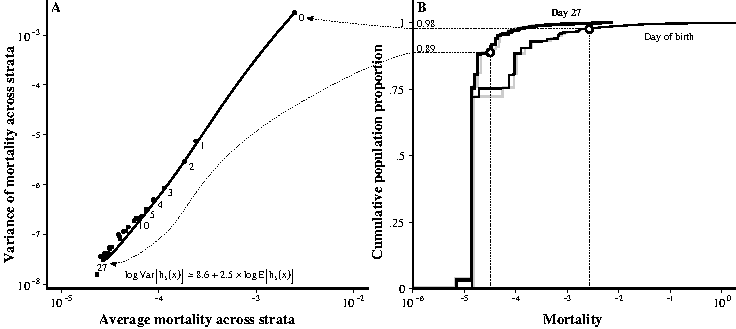
\includegraphics{fig/distribution_of_risk.pdf}
\caption{\label{fig:distribution-of-risk}Mean-variance relationship over day of age (A) and age-specific distribution function (B) of the mortality/hazard rates in a cohort of newborns across birth weight, gestational age, and Apgar score strata. The points in (A) mark mean and variance of the life table mortality rates, whereas the smooth line is the prediction from the Poisson regression. In plot (B), the gray lines refer to the life table estimates and the black lines to the model predictions.}
\end{figure}

\subsection{Shape and level of hazards are heterogeneous}\label{shape-and-level-of-hazards-are-heterogeneous}

The hazard trajectories predicted by the multilevel Poisson regression model \eqref{eq:themodel} closely match the mortality rate estimates from the life table. They reflect a high degree of heterogeneity among the 252 birth weight\(\times\)prematurity\(\times\)Apgar score strata of the U.S. 2009--2012 birth cohort (Figure \ref{fig:neonatal-hazard-trajectories}), varying both in level and shape. The heterogeneity is well illustrated by contrasting the lowest-low mortality subgroup (term-born infants with regular birth weight and an Apgar score of ten) with the highest-high mortality stratum (extremely premature infants with extremely low birth weight and an Apgar score of zero). At birth, the force of mortality ranges across five orders of magnitude with a hazard ratio of roughly 244,000 (!) between the extremes but over time hazards converge as there is a strong positive correlation between the level of the hazard at birth and the rate of mortality decline over the neonatal period. While the lowest-low mortality group features a comparatively flat hazard over age, declining by 39 percent over days 0 to 28, the hazard of the highest-high risk stratum drops by 99.8 percent over the same period. Hazard trajectories by Apgar score are stratified as expected on a low-high mortality continuum from ten to zero stretching multiple orders of magnitude within all birth weight \(\times\) prematurity combinations. However, hazards by Apgar score are clustered more closely among extremely preterm infants with extremely low birth-weight compared to term-born infants of regular or high birth weight.

The lack of proportionality in the hazard trajectories is evident in the varying pace of mortality decline over the first week of life. Thus, we can rule out the hypothesis of proportional frailties for the 252 sub-hazards along the birth weight\(\times\)prematurity\(\times\)Apgar score strata of the U.S. 2009--2012 birth cohort. Time-varying frailties as well as proportional unobserved frailties are however still consistent with our sample.

While the hazards are heterogeneous when compared directly, the majority of newborns are born on full-term, with regular birth weight and an Apgar score of nine. Thus the majority of the birth cohort is homogeneous with respect to their hazard trajectory.

\begin{figure}
\centering
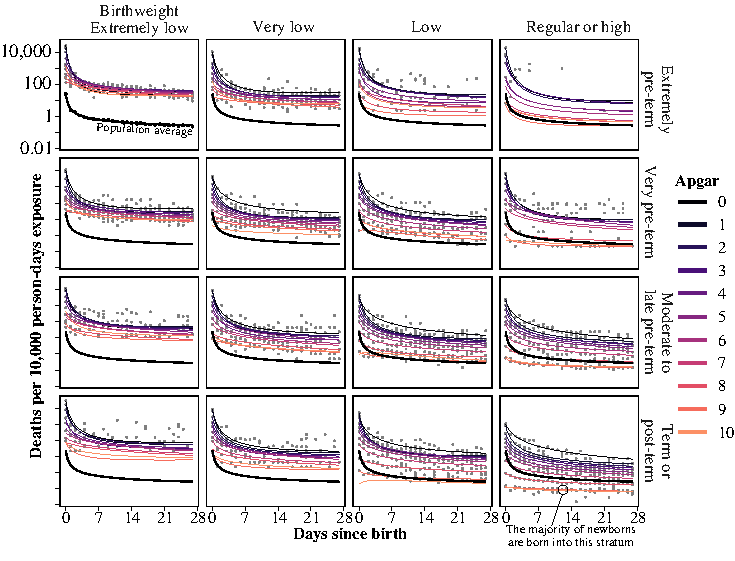
\includegraphics{fig/neonatal_hazard_trajectories.pdf}
\caption{\label{fig:neonatal-hazard-trajectories}Estimated hazard rates versus life table mortality rates over age by prematurity, birth weight, and Apgar score. There is substantial heterogeneity in the level and shape of the neonatal hazard trajectories. The lack of proportionality of the hazards is evident during the first week of life where the pace of mortality decline is positively correlated with the magnitude of mortality at birth. The black line in each panel shows the estimated hazard trajectory for the entire birth cohort.}
\end{figure}

\subsection{Mortality selection mainly acts shortly after birth}\label{mortality-selection-mainly-acts-shortly-after-birth}

Population-level mortality during the first day of life is ten times higher than mortality over the following day. This 90 percent mortality decline over 24 hours is mostly the result of a corresponding drop in the stratum specific mortality rates, which, on average, declined by 71 percent between both time points. The remaining 19 percent decline is explained by a change in population composition due to mortality selection on the day of birth. Over the following time intervals, mortality continues to decline at a fast pace with compositional effects ceasing to contribute substantially to this decline. At no point is the ratio of compositional mortality decline to total mortality decline \(\frac{\Delta \overline{m}_j^C}{\Delta \overline{m}_j}\) higher, or even near 0.5 (Table \ref{tab:tab-decomp-raw-rates}).

The results from the discrete-time life table analysis are mirrored by the Vaupel-Zhang decomposition of the hazard's rate of change at different ages. The contribution of mortality rate variance across strata to the slope in the hazard is around 23 percent at birth but merely 4.6 percent 24 hours later staying in the single digits over the remainder of the first month of life (Table \ref{tab:tab-vaupel-zhang}).

\begin{figure}
\centering
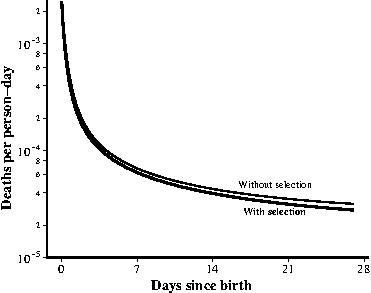
\includegraphics{fig/counterfactual_hazards.pdf}
\caption{\label{fig:counterfactual-hazards}Keeping the population composition fixed at the distribution observed at birth only results in a minor change of the population hazard trajectory.}
\end{figure}

In order to understand the impact of mortality selection on the overall shape of the hazard trajectory I compare the estimated population average hazard over age with a counterfactual population hazard based on the stratum specific hazard estimates of model \eqref{eq:themodel} but assuming the stratum specific population proportions to be fixed, thereby negating the effect of mortality selection on the population hazard. Figure \ref{fig:counterfactual-hazards} clearly shows that the steep decline in the risk of death following birth is not explained by selection due to differential mortality along the birth weight, Apgar score, and prematurity strata. However, mortality selection has some noticeable effect on the level of risk: Without selection, the hazard of death at day 28 would be an estimated 14 percent higher.

\begin{table}
\centering
\caption{\label{tab:tab-decomp-raw-rates}Direct and compositional components of mortality rate decline over the neonatal period.}
\centering
\begin{tabular}[t]{rrllllllll}
\toprule
Age & $\overline{m}_j$ &  & $\Delta \overline{m}_j$ & (\%) & $\Delta \overline{m}_j^D$ &  (\%) & $\Delta \overline{m}_j^C$ & (\%) & $\frac{\Delta \overline{m}_j^C}{\Delta \overline{m}_j}\%$\\
\midrule
0 & 2.5e-3 &  &  &  &  &  &  &  & \\
 &  & $\mapsto$ & -2.3e-3 & -90.4 & -1.8e-3 & -71.1 & -4.8e-4 & -19.2 & 21.3\\
1 & 2.4e-4 &  &  &  &  &  &  &  & \\
 &  & $\mapsto$ & -1.8e-4 & -73.4 & -1.7e-4 & -70.1 & -7.9e-6 & -3.3 & 4.5\\
7 & 6.4e-5 &  &  &  &  &  &  &  & \\
 &  & $\mapsto$ & -2.4e-5 & -37.8 & -2.3e-5 & -36.4 & -8.9e-7 & -1.4 & 3.7\\
14 & 4.0e-5 &  &  &  &  &  &  &  & \\
 &  & $\mapsto$ & -1.0e-5 & -25.9 & -1.0e-5 & -25.1 & -3.4e-7 & -0.9 & 3.3\\
21 & 2.9e-5 &  &  &  &  &  &  &  & \\
 &  & $\mapsto$ & -6.3e-6 & -21.3 & -6.1e-6 & -20.9 & -1.3e-7 & -0.4 & 2.1\\
27 & 2.3e-5 &  &  &  &  &  &  &  & \\
\bottomrule
\multicolumn{10}{l}{\textsuperscript{} Age refers to single day age groups.}\\
\end{tabular}
\end{table}

\begin{table}
\centering
\caption{\label{tab:tab-vaupel-zhang}Vaupel-Zhang decomposition of the slope in the hazard of death into direct and compositional components at selected ages.}
\centering
\begin{tabular}[t]{llllll}
\toprule
Age $x$ & $h(x)$ & $\dot{\overline{h}}(x)$ & $\overline{\dot{h}}(x)$ & $\sigma^2_h(x)$ & $\nu(x)\%$\\
\midrule
0 & 2.5e-3 & -1.2e-2 & -9.0e-3 & 2.8e-3 & 23.5\\
1 & 3.1e-4 & -3.0e-4 & -2.8e-4 & 1.4e-5 & 4.6\\
7 & 6.2e-5 & -6.1e-6 & -5.9e-6 & 1.8e-7 & 2.9\\
14 & 4.0e-5 & -1.7e-6 & -1.6e-6 & 6.1e-8 & 3.6\\
21 & 3.1e-5 & -7.9e-7 & -7.6e-7 & 3.7e-8 & 4.7\\
27 & 2.8e-5 & -4.7e-7 & -4.4e-7 & 3.1e-8 & 6.5\\
\bottomrule
\end{tabular}
\end{table}

\subsection{Stratum specific mortality converges}\label{stratum-specific-mortality-converges}

Following birth, the stratum specific mortality rates rapidly converge, explaining both the sudden decline in variance and mean-mode ratio of the mortality rate distribution (Figures \ref{fig:distribution-of-risk}, \ref{fig:mean-mode-convergence}).

\begin{figure}
\centering
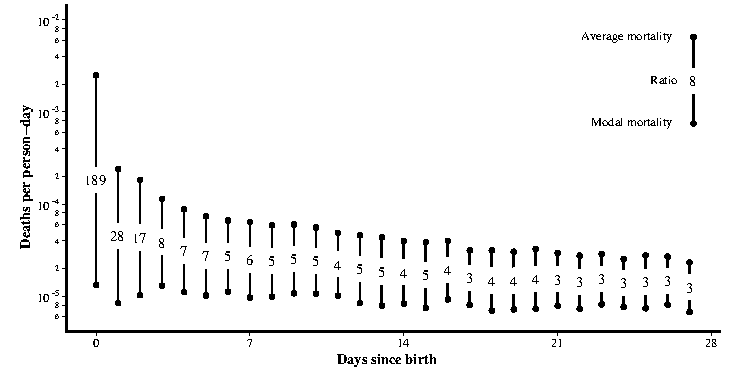
\includegraphics{fig/mean_mode_convergence.pdf}
\caption{\label{fig:mean-mode-convergence}The ratio of the population average and the modal mortality rates over the first four weeks of life. Following birth population mortality converges towards the low mortality of the most prevalent stratum (Apgar 9, Regular or high birth weight, born term or post-term) which is due to the convergence of high-risk strata.}
\end{figure}

The variance of death rates over strata is highest at birth and falls by more than 90 percent from day 0 to day 1 of age. The decline in variance is mainly the result of stratum specific death rates converging towards the population average, with only 19 percentage points decline explained by mortality selection. The mortality variance continues to decline substantially over the remainder of the first month of life, with mortality selection never contributing more than 4.5 percent to the total decline (Table \ref{tab:tab-decomp-raw-variances}).

During the first day of life, population mortality is 189 times higher than the mortality of the most prevalent stratum. This ratio declines by 85 percent over the next day of life, with only 20 percentage points of this decline explained by a shifting population composition. During the remainder of the neonatal period, mortality selection only minimally influences the continuing changes in the mean-mode mortality ratio, which eventually arrives at a value of around 3, a drop by 98 percent compared to the value at birth (Table \ref{tab:tab-memora-change}).

\begin{table}
\centering
\caption{\label{tab:tab-decomp-raw-variances}Direct and compositional components of mortality rate variance decline over the neonatal period.}
\centering
\begin{tabular}[t]{rrllllllll}
\toprule
Age & $v_j$ &  & $\Delta v_j$ & (\%) & $\Delta v_j^D$ &  (\%) & $\Delta v_j^C$ & (\%) & $\frac{\Delta v_j^C}{\Delta v_j^D}\%$\\
\midrule
0 & 2.5e-3 &  &  &  &  &  &  &  & \\
 &  & $\mapsto$ & -2.3e-3 & -90.4 & -1.8e-3 & -71.1 & -4.8e-4 & -19.2 & 21.3\\
1 & 2.4e-4 &  &  &  &  &  &  &  & \\
 &  & $\mapsto$ & -1.8e-4 & -73.4 & -1.7e-4 & -70.1 & -7.9e-6 & -3.3 & 4.5\\
7 & 6.4e-5 &  &  &  &  &  &  &  & \\
 &  & $\mapsto$ & -2.4e-5 & -37.8 & -2.3e-5 & -36.4 & -8.9e-7 & -1.4 & 3.7\\
14 & 4.0e-5 &  &  &  &  &  &  &  & \\
 &  & $\mapsto$ & -1.0e-5 & -25.9 & -1.0e-5 & -25.1 & -3.4e-7 & -0.9 & 3.3\\
21 & 2.9e-5 &  &  &  &  &  &  &  & \\
 &  & $\mapsto$ & -6.3e-6 & -21.3 & -6.1e-6 & -20.9 & -1.3e-7 & -0.4 & 2.1\\
27 & 2.3e-5 &  &  &  &  &  &  &  & \\
\bottomrule
\multicolumn{10}{l}{\textsuperscript{} Age refers to single day age groups.}\\
\end{tabular}
\end{table}

\begin{table}
\centering
\caption{\label{tab:tab-memora-change}Direct and compositional components of mean-mode ratio decline over the neonatal period.}
\centering
\begin{tabular}[t]{rrllllllll}
\toprule
Age & $r_j$ &  & $\Delta~r_{j}$ & (\%) & $\Delta~r_{j}^D$ &  (\%) & $\Delta~r_{j}^C$ & (\%) & $\frac{\Delta~r_{j}^C}{\Delta~r_{j}^D}\%$\\
\midrule
0 & 189 &  &  &  &  &  &  &  & \\
 &  & $\mapsto$ & -160 & -84.9 & -123 & -65.0 & -37 & -19.9 & 23.4\\
1 & 28 &  &  &  &  &  &  &  & \\
 &  & $\mapsto$ & -21 & -76.8 & -21 & -73.6 & 0 & -3.2 & 4.2\\
7 & 6 &  &  &  &  &  &  &  & \\
 &  & $\mapsto$ & -1 & -27.5 & -1 & -26.0 & 0 & -1.5 & 5.4\\
14 & 4 &  &  &  &  &  &  &  & \\
 &  & $\mapsto$ & -1 & -22.1 & -1 & -21.2 & 0 & -0.9 & 3.9\\
21 & 3 &  &  &  &  &  &  &  & \\
 &  & $\mapsto$ & 0 & -7.6 & 0 & -7.2 & 0 & -0.5 & 6.2\\
27 & 3 &  &  &  &  &  &  &  & \\
\bottomrule
\multicolumn{10}{l}{\textsuperscript{} Age refers to single day age groups.}\\
\end{tabular}
\end{table}

\section{Discussion}\label{discussion}

Frailty theory cautions us against taking the population level hazard shape as representative for the risk trajectory of the population members. The analysis of neonatal mortality indeed clearly demonstrates the potential severity of this ecological fallacy, with the majority of newborns experiencing a hazard trajectory radically different from what is observed on the aggregate level. Yet, this difference does not arise from mortality selection but from the non-proportionality of stratum specific hazards. Neonatologists know that the first 24 hours of life are the most critical in determining the further survival of the preterm infant. Once the one-day threshold is passed, the survival chances not only drastically improve but, as shown in this paper, converge towards the survival chances of healthy term-born infants. The popular proportional frailty model is severely misspecified for situations where an individual may be saved due to medical intervention, i.e., where the physiological state of an individual and thus the associated frailty changes abruptly. In consequence, even if the model fits the aggregate age pattern well, as it does in case of the Hougaard-Gompertz fit to the age trajectory of infant mortality (Figure \ref{fig:hougaard-gompertz-fit}), inferences drawn from it are biased.

To escape the strong assumptions of frailty models, I based the analysis in this paper on the \emph{observed} heterogeneity in age-specific mortality across mutually exclusive population strata but, in turn, left open the possibility for \emph{hidden} heterogeneity within a particular stratum. This \emph{hidden} heterogeneity would need to be of extraordinary magnitude in order to explain the observed pace of mortality decline via mortality selection -- note that the heterogeneity observed in this paper spans five orders of magnitude and hardly shapes the overall hazard via selection -- and is thus unlikely to be found in social strata, which rarely exceed single digit hazard ratios. However, a further division of the population along the presence and severity of congenital malformations may uncover that the mortality decline following birth is primarily the effect of the vanishing subpopulation of newborns featuring congenital disabilities incompatible with life. While this particular hypothesis can be tested in a future publication, one can never exclude the possibility of further unobserved quantities influencing observed outcomes. All that can be confidently said based on the data analyzed above is that the heterogeneity in risk along birth weight, Apgar score, and prematurity has only a minimal impact on the shape of the population level age trajectory of neonatal mortality.

The discipline of neonatology has achieved great successes in pushing the limit of viability to earlier gestational ages. Whereas in 1971 newborns younger than 28 weeks or weighing less than 1000 grams were given no realistic chance of survival \citep{Malloy2022}, recently, two-year survival probabilities for infants delivered at US hospitals at 23 weeks have exceeded 50\% if active treatment was given \citep{Bell2022}. From the perspective of mortality selection one may wonder if the improved survival of extremely premature infants leads to increased cohort mortality at later ages. While I did not address this question directly, the results of this study indicate that mortality selection only has a weak effect on the level and shape of the cohort hazard past the first day of life. This is because mortality selection primarily acts on the day of birth with the hazards of the frailest subgroups dropping to safer levels within hours of birth. Globally it has been shown that lower under-5 mortality goes hand in hand with a compression of mortality towards the neonatal ages \citep{Hug2019}. This finding is consistent with an intervention practice which both successfully addresses risk factors which contribute to post-neonatal mortality, such as infections, and successfully distinguishes between infants which, given active treatment, will survive to childhood, and those who most likely will not.

A peculiar finding is the near-perfect power-law relationship between the mean and the variance of the distribution of stratum-specific mortality rates over age -- a further example of ``Taylor's law'' in demography: Analyzing data on the spatial distribution of various species \citet{Taylor1961} observed that the variance in population count per unit area is well predicted by a power of the average population count. Similar mean-variance relationships have been found for population densities in human populations \citep{Cohen2013, Naccarato2018} and recently for time-series of age-specific mortality rates and rates of mortality improvement \citep{Bohk2015, Cohen2018}. Whereas the studies by Cohen, Bohk, and Rau are based on the concept of a ``temporal mean/variance,'' i.e., mean and variance are estimated from observations repeated over age or period, I contribute the first demonstration of Taylor's law in human mortality based on the distribution of risk at any single point in time within a cohort of individuals followed over age.

\section{Conclusion}\label{conclusion}

The sudden drop in population mortality following birth is predominantly the result of stratum specific hazard rates quickly converging towards rather low levels. The compositional shift in the population resulting from mortality selection only has a minimal impact on the age trajectory of neonatal mortality.

Hazard trajectories in the first days following birth are highly non-proportional between risk strata. Thus the common assumption of proportionality, as in the popular Cox model, may lead to biased estimates in the study of neonatal mortality.

It remains to be seen if the simple Taylor's law expression that describes the time-evolution of mean and variance in mortality among a cohort of newborns replicates in other populations and at other ages. The prospect of having a 2-parameter expression for the mortality dynamics in a heterogeneous aging cohort may motivate future inquiries in that direction.

\section{Acknowledgments}\label{acknowledgments}

Foo.

%--- Print references --------------------------------------------------

\newpage

\addcontentsline{toc}{section}{\numberline{}References}

\bibliography{refs.bib}

%--- Print appendix ----------------------------------------------------

% total number of appendices
\newcounter{totalappendixcount}  \stepcounter{totalappendixcount}  \stepcounter{totalappendixcount}  \stepcounter{totalappendixcount} 
% loop iterator
\newcounter{currentappendixcount}

% add appendices

 \stepcounter{currentappendixcount}
 % if only a single appendix use a different labeling scheme
 \ifnum\value{totalappendixcount}=1
   \def \currentappendixlabel {}
   \def \currentappendixfloatlabel {A}
 \else
   \def \currentappendixlabel {\Alph{currentappendixcount}}
   \def \currentappendixfloatlabel {\Alph{currentappendixcount}}
 \fi

  \clearpage
  \section*{Appendix \currentappendixlabel}\FloatBarrier
  \addcontentsline{toc}{section}{\numberline{}Appendix \currentappendixlabel}
  \setcounter{section}{0}
  \renewcommand{\thesection}{\currentappendixfloatlabel-\arabic{section}}
  \setcounter{figure}{0}
  \renewcommand{\thefigure}{\currentappendixfloatlabel-\arabic{figure}}
  \setcounter{table}{0}
  \renewcommand{\thetable}{\currentappendixfloatlabel-\arabic{table}}

  \textbf{The Hougaard-Gompertz frailty model.}
  Let the hazard of death at age \(x\) for a newborn with frailty \(z\) be \(h_z(x|z)=zh_0(x)\) with \(z\) drawn from the three parameter frailty distribution proposed by \citet{Hougaard1986} denoted with \(Z \sim \text{Houg}(x; \alpha, \delta, \theta)\) and Gompertz baseline hazard \(h_0(x)=ae^{bx}\) with corresponding cumulative hazard \(H_0(x) = \int_0^x h_0(s)\,\text{d}s=a(e^{bx}-1)/b\). The average frailty among the survivors at \(x\) then is \(\text{E}[Z|X\geq x]=\delta\left(\theta + H_0(x)\right)^{\alpha -1}\) \citep[393]{Hougaard1986}. Substituting \(\delta = \frac{1} {\theta^{\alpha-1}}\) eliminates one parameter from the model and fixes the average frailty at birth at one. The population hazard then is

  \[
  h(x)=\text{E}[Z|X=x]h_0(x)=\left(\frac{\theta +   a(e^{bx}-1)/b}{\theta}\right)^{\alpha -1}ae^{bx},
  \]

  with log-hazard

  \[
  \log h(x) =
  (\alpha-1)\log\left(\frac{\theta + a(e^{bx}-1)/b}{\theta}\right) +
  \log a + bx
  \]

  The above hazard is fitted to daily death counts \(D_j\) and exposure times \(E_j\) of the U.S. 2009--2012 infant life table via a Bayesian non-linear Poisson regression model

  \[
  \begin{aligned}
  D_j &\sim \text{Pois}(\lambda_jE_j)~\text{for}~j=1,\ldots,365 \\
  \lambda_j &= e^{\log h(x_j;a,b,\theta,\alpha)}
  \end{aligned}
  \]

  with parameter transformations

  \[
  \begin{aligned}
  a &= e^{\beta_0} \\
  b &= \beta_1 \\
  \theta &= e^{\beta_2} \\
  \alpha &= \log\frac{\beta_3}{1-\beta_3},
  \end{aligned}
  \]

  and priors

  \[
  \begin{aligned}
  \beta_0 &\sim \text{N}(-8, 1) \\
  \beta_1 &\sim \text{N}(-0.03, 1) \\
  \beta_2 &\sim \text{N}(-6, 1) \\
  \beta_3 &\sim \text{N}(0.5, 1).
  \end{aligned}
  \]


 \stepcounter{currentappendixcount}
 % if only a single appendix use a different labeling scheme
 \ifnum\value{totalappendixcount}=1
   \def \currentappendixlabel {}
   \def \currentappendixfloatlabel {A}
 \else
   \def \currentappendixlabel {\Alph{currentappendixcount}}
   \def \currentappendixfloatlabel {\Alph{currentappendixcount}}
 \fi

  \clearpage
  \section*{Appendix \currentappendixlabel}\FloatBarrier
  \addcontentsline{toc}{section}{\numberline{}Appendix \currentappendixlabel}
  \setcounter{section}{0}
  \renewcommand{\thesection}{\currentappendixfloatlabel-\arabic{section}}
  \setcounter{figure}{0}
  \renewcommand{\thefigure}{\currentappendixfloatlabel-\arabic{figure}}
  \setcounter{table}{0}
  \renewcommand{\thetable}{\currentappendixfloatlabel-\arabic{table}}

  \textbf{The quadratic hazard over log age.}
  Quadratic relationships between log age and log mortality can be captured by the expression

  \[
  h(x) = e^{\beta_0 + \beta_1\log(x+1)+\beta_2\log^2(x+1)},
  \]

  with derivative wrt. \(x\)

  \[
  h'(x) = (x+1)^{\beta_1-1}e^{\beta_0+\beta_2\log^2(x+1)}\left(\beta_1+2\beta_2\log(x+1)\right),
  \]

  and survival function

  \[
  S(x) 
     = \exp\left(\frac {
       \sqrt{\pi}\exp\left(b_{0}-\frac{(b_{1}+1)^2}{4b_{2}}\right)
       \left(\text{erfi}\left(\frac{b_{1}+1}{2\sqrt{b_{2}}}\right) -
       \text{erfi}\left(\frac{b_{1}+2b_{2}\log(x+1)+1}{2\sqrt{b_{2}}}\right)
       \right)
     } {
       2\sqrt{b_{2}}
     }\right).
  \]

  An efficient algorithm for the evaluation of the imaginary error function \(\text{erfi}(x)=\frac{2}{\sqrt{\pi}}\int_0^{x} \text{exp}\left(t^2\right)\,\text{d}t\) exists \citep{Poppe1990} and is implemented in the \texttt{C++} library \texttt{Faddeeva} which can be called from within \texttt{R} via the package \texttt{RcppFaddeeva}.


 \stepcounter{currentappendixcount}
 % if only a single appendix use a different labeling scheme
 \ifnum\value{totalappendixcount}=1
   \def \currentappendixlabel {}
   \def \currentappendixfloatlabel {A}
 \else
   \def \currentappendixlabel {\Alph{currentappendixcount}}
   \def \currentappendixfloatlabel {\Alph{currentappendixcount}}
 \fi

  \clearpage
  \section*{Appendix \currentappendixlabel}\FloatBarrier
  \addcontentsline{toc}{section}{\numberline{}Appendix \currentappendixlabel}
  \setcounter{section}{0}
  \renewcommand{\thesection}{\currentappendixfloatlabel-\arabic{section}}
  \setcounter{figure}{0}
  \renewcommand{\thefigure}{\currentappendixfloatlabel-\arabic{figure}}
  \setcounter{table}{0}
  \renewcommand{\thetable}{\currentappendixfloatlabel-\arabic{table}}

  \textbf{The Vaupel-Zhang equality.}
  I find it instructive to derive the Vaupel-Zhang equality from a simple finite mixture distribution of survival times as it gives justification to the weighted averages employed in this paper. Once the marginal hazard rate has been shown to be a weighted average of hazards among the survivors the proof is the same as \citet{Vaupel2010a}.

  Let \(X\) be the positive real-valued random variable ``age at death'' and \(K\) be a random index denoting membership to the \(k\)th population stratum. The marginal density of ages at death is given by the discrete mixture distribution

  \[
  f(x)=\sum_k f(x|k)\mathrm{P}(k),
  \]

  where \(f(x|k)\) is the conditional density of deaths and \(\mathrm{P}(k)\) the probability of membership in stratum \(k\). By definition the conditional and marginal survival functions are

  \[
  \begin{aligned}
  S(x|k) &= \mathrm{P}(X>x|k) = \int_x^\infty f(x|k)\,\text{d}x \\
  S(x) &= \mathrm{P}(X>x) = \int_x^\infty f(x)\,\text{d}x,
  \end{aligned}
  \]

  which give rise to the conditional and marginal hazards via the relationships

  \[
  \begin{aligned}
  h(x|k) &= -S'(x|k)/S(x|k)\\
  h(x) &= -S'(x)/S(x),
  \end{aligned}
  \]

  where the prime mark denotes the derivative with respect to age \(x\).

  The Vaupel-Zhang equality states that for the survivors at age \(x\) the age-derivative of their average hazard is equal to the average age derivative minus the variance of the hazards, in their notation

  \[
  \dot{\overline{h}}(x) = \overline{\dot{h}}(x) - \sigma_h^2(x),
  \]

  where

  \[
  \begin{aligned}
    \dot{\overline{h}}(x) &= \left[\sum_k h(x|k)\mathrm{P}(k|X>x)\right]' \\
    \overline{\dot{h}}(x) &= \sum_k h'(x|k)\mathrm{P}(k|X>x) \\
    \sigma_h^2(x) &=
      \sum_k h(x|k)^2 \mathrm{P}(k|X>x) -
      \left[\sum_k h(x|k)\mathrm{P}(k|X>x)\right]^2.
  \end{aligned}
  \]

  \textbf{Proof:}

  Bayes Theorem gives the probability of being in stratum \(k\) given survival to age \(x\) as

  \[
  \mathrm{P}(k|X>x) = \frac{\mathrm{P}(X>x|k)\mathrm{P}(k)} {\mathrm{P}(X>x)} =     \frac{S(x|k)\mathrm{P}(k)}{S(x)}
  \]

  The marginal survival \(S(x)\) can be calculated from conditional survival \(S(x|k)\) and stratum distribution \(\mathrm{P}(k)\) via the law of total probability as

  \[
  \begin{aligned}
  S(x) &= \mathrm{P}(X>x) \\
  &= \sum_k \mathrm{P}(X>x|k)\mathrm{P}(k) \\
  &= \sum_kS(x|k)\mathrm{P}(k),
  \end{aligned}
  \]

  with age derivative

  \[
  \begin{aligned}
    S'(x) &= \sum_k S'(x|k)\mathrm{P}(k) \\
          &= \sum_k -h(x|k)S(x|k)\mathrm{P}(k).
  \end{aligned}
  \]

  By substituting \(S'(x)\) into \(h(x)=-\frac{S'(x)}{S(x)}\) one can express the marginal hazard as a weighted average of the hazards of the survivors:

  \[
  \begin{aligned}
    h(x) &= -\frac{\sum_k -h(x|k)S(x|k)\mathrm{P}(k)} {S(x)} \\
         &= \sum_k \frac{h(x|k)S(x|k)\mathrm{P}(k)} {S(x)} \\
         &= \sum_k h(x|k)\mathrm{P}(k|X>x).
  \end{aligned}
  \]

  Taking the derivative of \(h(x)\) gives

  \[
  \begin{aligned}
  \dot{\overline{h}}(x) &=
  \sum_k h'(x|k)\mathrm{P}(k|X>x) + \sum_k h(x|k)\mathrm{P}'(k|X>x) \\
      &= \overline{\dot{h}}(x) +
      \sum_k h(x|k)\mathrm{P}'(k|X>x).
  \end{aligned}
  \]

  The second term can be manipulated to yield

  \[
  \begin{aligned}
    \sum_k h(x|k)\mathrm{P}'(k|X>x) &=
    \sum_k h(x|k) \left(
        \frac {\mathrm{P}(k)S'(x|k)} {S(x)} -
        \frac {\mathrm{P}(k)S'(x)S(x|k)} {S(x)^2}
      \right) \\
    &=
    \sum_k \frac {h(x|k)\mathrm{P}(k)S'(x|k)} {S(x)} -
    \sum_k \frac {h(x|k)\mathrm{P}(k)S'(x)S(x|k)} {S(x)^2}  \\
    &=
    \sum_k \frac {h(x|k) \mathrm{P}(k)S'(x|k)} {S(x)} -
    \frac {S'(x)} {S(x)} \sum_k h(x|k) \mathrm{P}(k|X>x) \\
    &=
    \sum_k \frac {h(x|k) \mathrm{P}(k)S'(x|k)} {S(x)} - h(x)^2 \\
    &=
    \sum_k \frac {-h(x|k)^2 \mathrm{P}(k)S(x|k)} {S(x)} - h(x)^2 \\
    &=
    -\sum_k h(x|k)^2 \mathrm{P}(k|X>x) - h(x)^2 \\
    &= 
    -\sigma^2_h(x),
  \end{aligned}
  \]

  completing the proof.


%--- End document ------------------------------------------------------

\cleardoublepage

\end{document}
